\documentclass[handout]{ximera}
%handout:  for handout version with no solutions or instructor notes
%handout,instructornotes:  for instructor version with just problems and notes, no solutions
%noinstructornotes:  shows only problem and solutions

%% handout
%% space
%% newpage
%% numbers
%% nooutcomes

%I added the commands here so that I would't have to keep looking them up
%\newcommand{\RR}{\mathbb R}
%\renewcommand{\d}{\,d}
%\newcommand{\dd}[2][]{\frac{d #1}{d #2}}
%\renewcommand{\l}{\ell}
%\newcommand{\ddx}{\frac{d}{dx}}
%\everymath{\displaystyle}
%\newcommand{\dfn}{\textbf}
%\newcommand{\eval}[1]{\bigg[ #1 \bigg]}

%\begin{image}
%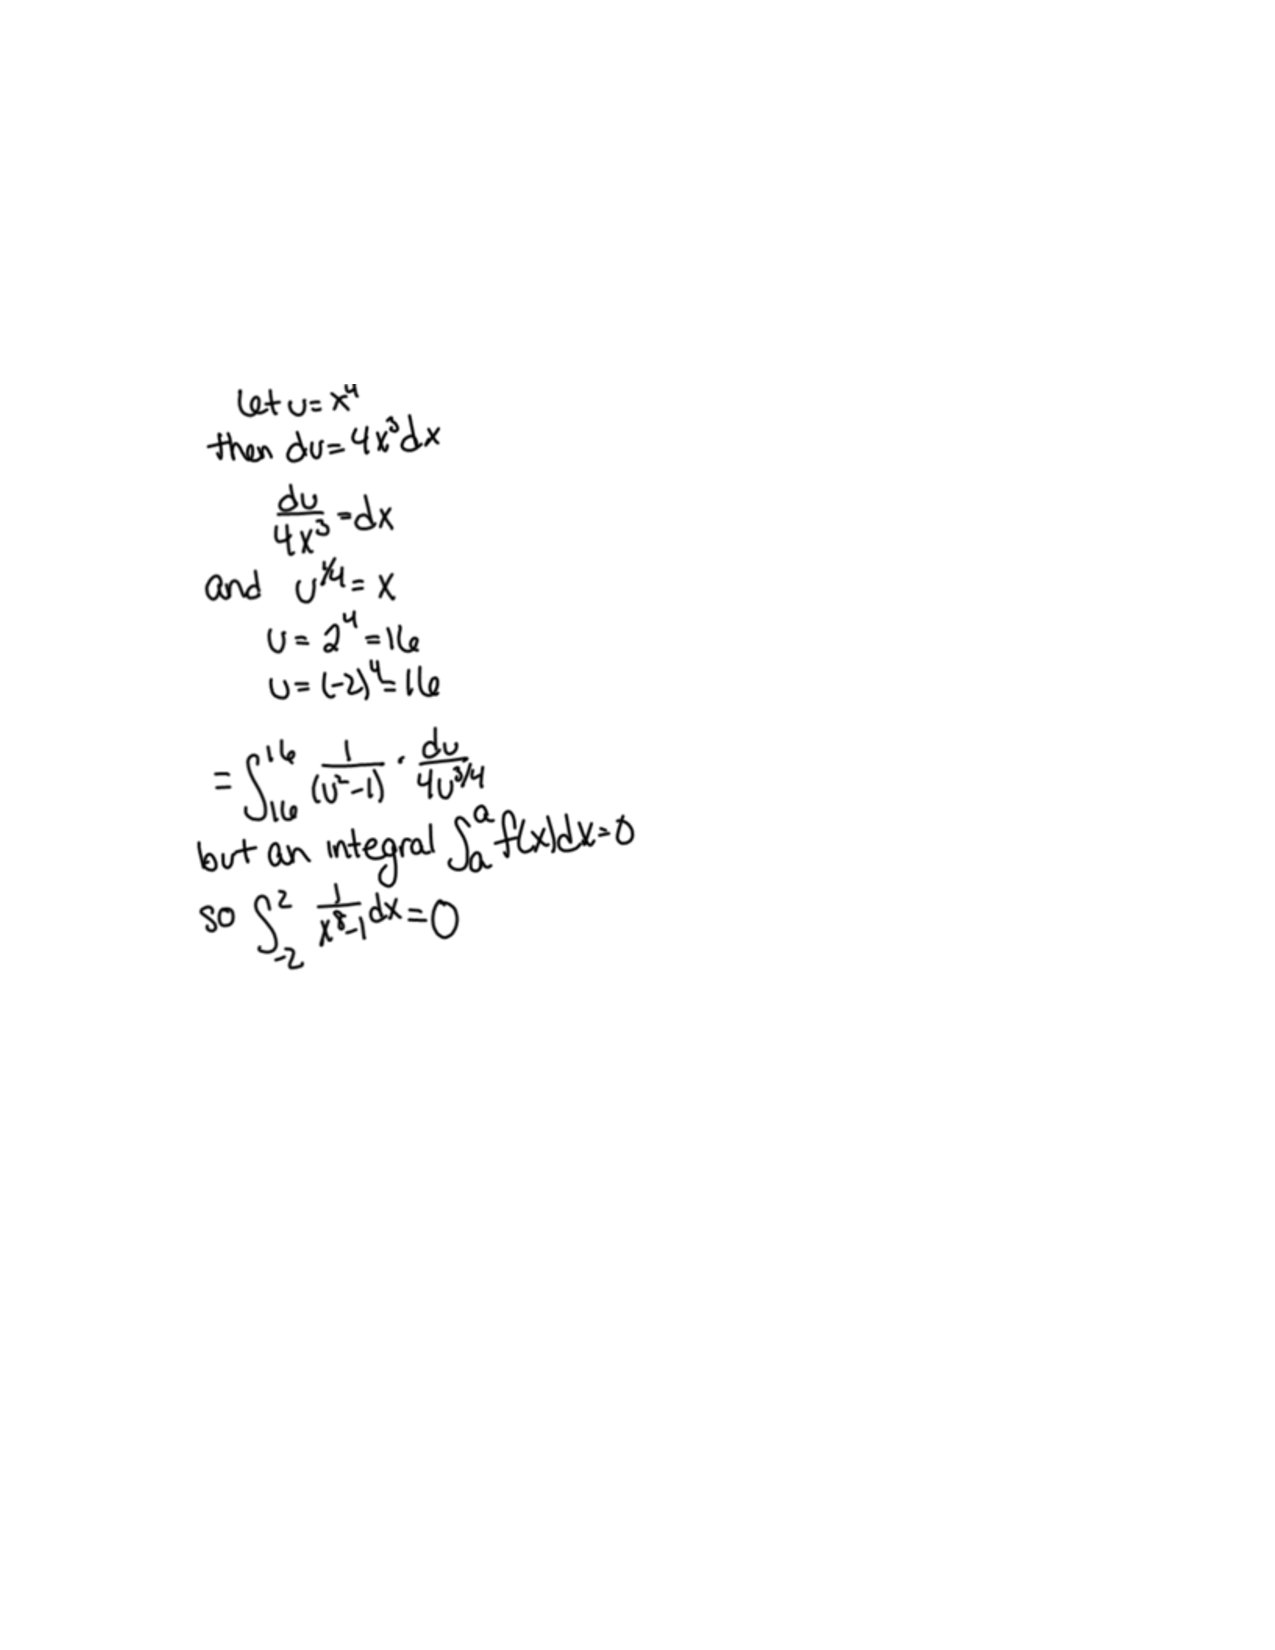
\includegraphics[trim= 170 420 250 180]{Figure1.pdf}
%\end{image}

%add a ``.'' below when used in a specific directory.
\newcommand{\RR}{\mathbb R}
\renewcommand{\d}{\,d}
\newcommand{\dd}[2][]{\frac{d #1}{d #2}}
\renewcommand{\l}{\ell}
\newcommand{\ddx}{\frac{d}{dx}}
\newcommand{\dfn}{\textbf}
\newcommand{\eval}[1]{\bigg[ #1 \bigg]}

\usepackage{multicol}

\renewenvironment{freeResponse}{
\ifhandout\setbox0\vbox\bgroup\else
\begin{trivlist}\item[\hskip \labelsep\bfseries Solution:\hspace{2ex}]
\fi}
{\ifhandout\egroup\else
\end{trivlist}
\fi} %% we can turn off input when making a master document

\title{Recitation \#18: Comparison Tests and Alternating Series}  

\begin{document}
\begin{abstract}		\end{abstract}
\maketitle




%Problem 1
\begin{problem}
Determine if the following series absolutely converge, conditionally converge, or diverge.
	%\begin{multicols}{2}
	\begin{enumerate}
	
	\item  $\sum_{n=0}^\infty \frac{(-1)^n}{n+3}$
	
	\item  $\sum_{n=1}^\infty \frac{(-1)^n (n+1)^n}{(2n)^n}$
	
	\item  $\sum_{n=1}^\infty (-1)^{n+1} n^2 e^{\frac{-n^3}{3}}$
	
	\item  $\sum_{n=0}^\infty \frac{(-1)^n \cdot 5}{3^n + 3^{-n}}$
	
	\item  $\sum_{n=4}^\infty \frac{(-2)^n}{n}$
	
	\item  $\sum_{n=0}^\infty \frac{n^2+2n+1}{3n^4+1}$
	
	\item  $\sum_{n=1}^\infty \left[ \left( 1+\frac{1}{n} \right)^2 e^{-n} \right]$
	
	\end{enumerate}
	%\end{multicols}
	
	\begin{freeResponse}
	
	\begin{enumerate}
	
	\item  Since $\frac{1}{n+3}$ is positive and decreasing, the Alternating Series Test applies.  
	Thus, this series converges.  
	But we know that $\sum_{n=1}^\infty \frac{1}{n+3}$ diverges (Harmonic Series) and so $\sum_{n=0}^\infty \frac{(-1)^n}{n+3}$ is {\color{red}conditionally convergent}.
	
	\item  Let $a_n = \frac{(n+1)^n}{(2n)^n}$.  
	Applying the Root Test, we see that
		\begin{align*}
		\lim_{n \to \infty} \sqrt[n]{a_n} &= \lim_{n \to \infty} \frac{n+1}{2n}  \\
		&= \frac{1}{2} < 1.
		\end{align*}
	So $\sum_{n=1}^\infty \frac{(n+1)^n}{(2n)^n}$ converges, and therefore $\sum_{n=1}^\infty \frac{(-1)^n (n+1)^n}{(2n)^n}$ is {\color{red}absolutely convergent}.
	
	\item  Let $f(x) = x^2 e^{\frac{-x^3}{3}}$.  
	The function $f(x)$ is continuous, positive, and decreasing.  
	So we apply the integral test
		\begin{align*}
		\int_1^\infty x^2 e^{\frac{-x^3}{3}} \d x
		&= \lim_{b \to \infty} \int_1^b x^2 e^{\frac{-x^3}{3}} \d x  \\
		&= \lim_{b \to \infty} \int_{\frac{1}{3}}^{\frac{b^3}{3}} e^{-u} \d u \qquad {\color{red}u=\frac{x^3}{3}, \, \d u = x^2 \d x}  \\
		&= \lim_{b \to \infty} \left[ -e^{\frac{-b^3}{3}} + e^{\frac{-1}{3}} \right]  \\
		&= 0 + e^{\frac{-1}{3}} = e^{\frac{-1}{3}}.
		\end{align*}
	So, by the Integral Test, $\sum_{n=1}^\infty n^2 e^{\frac{-n^3}{3}}$ converges.  
	Therefore, $\sum_{n=1}^\infty (-1)^{n+1} n^2 e^{\frac{-n^3}{3}}$ is {\color{red}absolutely convergent}.
	
	\item  First, notice that
		\[
		\frac{5}{3^n} > \frac{5}{3^n + 3^{-n}}.
		\]
	Then since $\sum_{n=0}^\infty \frac{5}{3^n}$ converges (geometric series with $r = \frac{1}{3} < 1$), we know that 
	$\sum_{n=0}^\infty \frac{5}{3^n + 3^{-n}}$ converges by the Comparison Test.  
	Thus, the series $\sum_{n=0}^\infty \frac{(-1)^n \cdot 5}{3^n + 3^{-n}}$ is {\color{red}absolutely convergent}.
	
	\item  Since the sequence $\left\{ \frac{(-2)^n}{n} \right\}$ diverges, the series $\sum_{n=4}^\infty \frac{(-2)^n}{n}$ {\color{red}diverges} by the Divergence Test.
	
		\item  Notice that all the terms of this series are positive.  Use the \dfn{Limit Comparison Test} with $\sum_{n=1}^\infty \frac{1}{n^2}$.
			\begin{align*}
			\lim_{n \to \infty} \frac{a_n}{b_n}
			&= \lim_{n \to \infty} \frac{n^2+2n+1}{3n^4+1} \cdot \frac{n^2}{1}  \\
			&= \frac{1}{3}.
			\end{align*}
			
		Therefore, since $\sum_{n=1}^\infty \frac{1}{n^2}$ converges, by the Limit Comparison Test we know that $\sum_{n=0}^\infty \frac{n^2+2n+1}{3n^4+1}$ converges and therefore is {\color{red}absolutely convergent}.
		
	
		
		\item  Notice that all the terms of this series are positive. Use the \dfn{Comparison Test} with $\sum_{n=1}^\infty 2 \cdot e^{-n}$.
		
		First, notice that for all $n \geq 3$,
			\[
			\left( 1 + \frac{1}{n} \right)^2 < 2.
			\]		
		Also, notice that $\sum_{n=1}^\infty e^{-n}$ is a convergent geometric series.  
		Therefore $\sum_{n=1}^\infty 2 \cdot e^{-n}$ converges, and so $\sum_{n=1}^\infty \left[ \left( 1+\frac{1}{n} \right)^2 e^{-n} \right]$ converges by the Comparison Test and therefore is {\color{red}absolutely convergent}.
		
	
	\end{enumerate}
	
	\end{freeResponse}
	
\end{problem}

\begin{instructorNotes}
These problems use a mix of tests.  
One of the main goals is for students to get practice determining which test to use.
	\begin{enumerate}
	\item  Limit Comparison Test with the harmonic series
	\item  Root Test
	\item  Integral Test
	\item  Limit Comparison Test
	\item  Divergence Test.  
	Be sure to talk about ``pulling out the $-1$'' to get an alternating series in standard form.  
	Talk about how the Alternating Series Test and the Divergence Test will take care of conditional convergence for most (but not all) alternating series that they will see.
	\end{enumerate}
\end{instructorNotes}







%problem 2
\begin{problem}
\begin{enumerate}

\item  Find an upper bound for how close $\sum_{k=0}^4 \frac{(-1)^k k}{4^k}$ is to the value of $\sum_{k=0}^\infty \frac{(-1)^k k}{4^k}$.

\item  (Calculator Recommended) How many terms are needed to estimate $\sum_{n=1}^\infty \frac{(-1)^n \ln n}{n!}$ to within $10^{-6}$?

\end{enumerate}
	\begin{freeResponse}
	\begin{enumerate}

	\item  Recall from the lesson that the remainder $R_n$ is given by
		\[
		R_n = |S - S_n| \leq a_{n+1}.
		\]
	Also notice that
		\[
		\sum_{k=0}^\infty \frac{(-1)^k k}{4^k} = \sum_{k=1}^\infty \frac{(-1)^{k-1} (k-1)}{4^{k-1}}
		\]
	and
		\[
		\sum_{k=0}^4 \frac{(-1)^k k}{4^k} = \sum_{k=1}^5 \frac{(-1)^{k-1} (k-1)}{4^{k-1}}.
		\]
	So
		\begin{align*}
		&\biggr| \sum_{k=0}^\infty \frac{(-1)^k k}{4^k} - \sum_{k=0}^4 \frac{(-1)^k k}{4^k} \biggr|  \\
		&= \biggr| \sum_{k=1}^\infty \frac{(-1)^{k-1} (k-1)}{4^{k-1}} - \sum_{k=1}^5 \frac{(-1)^{k-1} (k-1)}{4^{k-1}} \biggr|  \\
		&= | S - S_5 |  \\
		&= R_6 \leq a_6 = \boxed{\frac{5}{4^5}}
		\end{align*}

	\item  Since $R_n \leq a_{n+1}$, we need to find $n$ so that 
		\begin{align*}
		&a_{n+1} \leq 10^{-6}  \\
		\Longleftrightarrow 	\qquad	&\frac{\ln (n+1)}{(n+1)!} \leq 10^{-6}  \\
		\Longleftrightarrow 	\qquad	&\frac{(n+1)!}{\ln (n+1)} \geq 10^6 
		\end{align*}
	Using a calculator, we see that this inequality holds for $n \approx 8.8$.  
	So for $\boxed{n \geq 9}$, $R_n < 10^{-6}$.  

	\end{enumerate}
	\end{freeResponse}
		
\end{problem}

\begin{instructorNotes}
Split (a) and (b) among the groups.
\end{instructorNotes}









	
	
	
	
	
	
	
	
	

	










								
				
				
	














\end{document} 


















